\documentclass{beamer}

\usepackage{multicol}
\usepackage{amssymb}


\title{Nix/NixOS/Nixpkgs}
\subtitle{
\includegraphics[width=0.3\textwidth]{nixos.png} \\ Made with Nix, $\heartsuit$, and \LaTeX}
\author{Ethan Carter Edwards \\ ethanedwards@college.harvard.edu}
\date{February 21, 2026}
\beamertemplatenavigationsymbolsempty


\begin{document}

\frame{\titlepage}

\begin{frame}

\frametitle{Who am I?}

My name is Ethan Edwards. I've been heavily involved with the project for the past few years and interned with the NixOS foundation last summer. Here are some statistics outlining my contributions upstream:

\begin{enumerate}
    \item 286 Packages maintained
    \item 229 PRs merged
    \item 30+ modules/integration tests written
    \item 1400+ PRs reviewed
    \item 216 PRs otherwise commented on
    \item 407 PRs otherwise involved with
    \item Maintainer for the NGI and Darwin (MacOS) teams
    \item Converted countless people to Nix :)
\end{enumerate}

\end{frame}

\begin{frame}


\begin{multicols}{2}

Nix is the brainchild of Eelco Dolstra. He started the project more than 20 years ago as his PhD thesis. While he has remained heavily involved, he is no longer the technical lead.


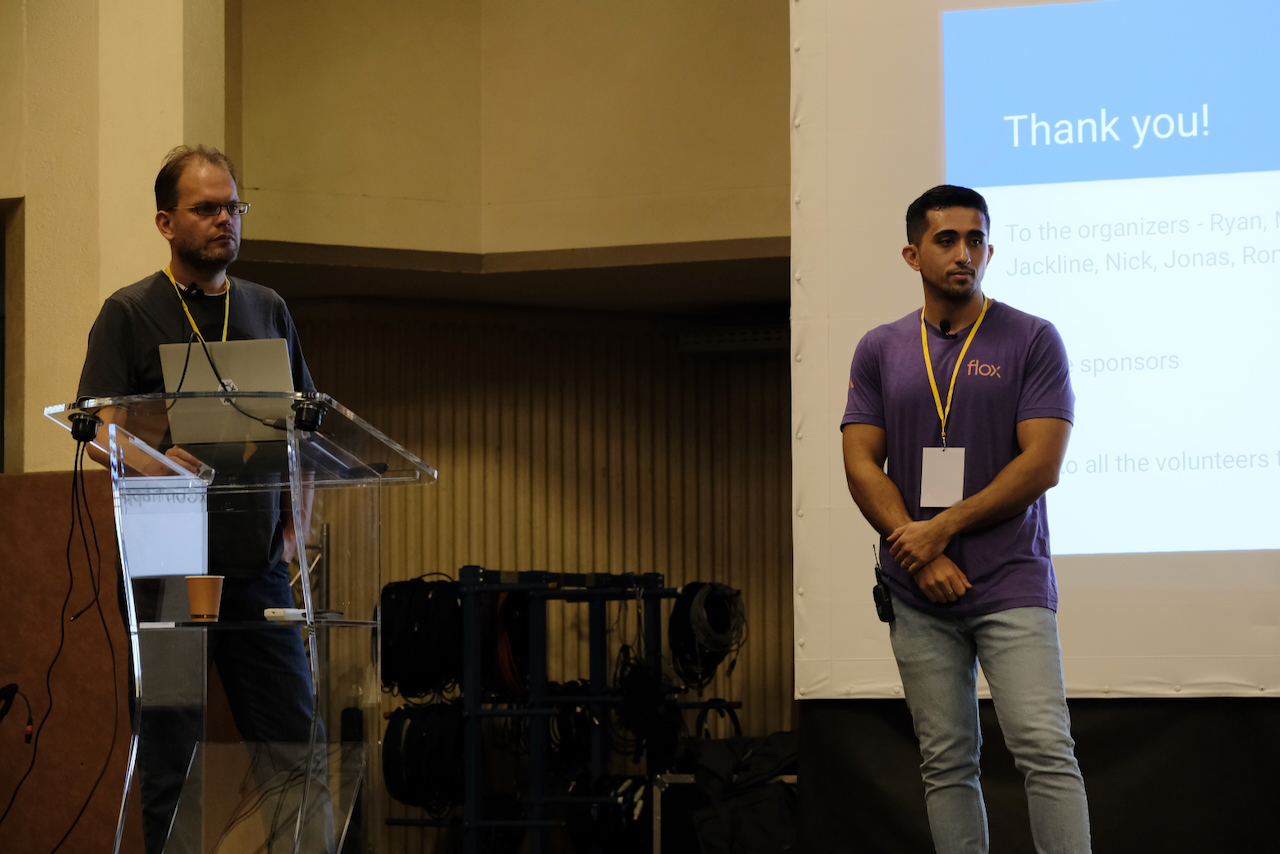
\includegraphics[width=0.6\textwidth]{ronandeelco.jpeg}

\end{multicols}

\end{frame}

\begin{frame}

\frametitle{Goals for this talk:}

\begin{multicols}{2}
\begin{enumerate}
    \item Introduce the Nix DSL
    \item Introduce the Nixpkgs repository
    \item Introduce the Linux Distro NixOS
    \item Show my use cases/Nix in action
    \item Convert you all to Nix! (world domination)
\end{enumerate}

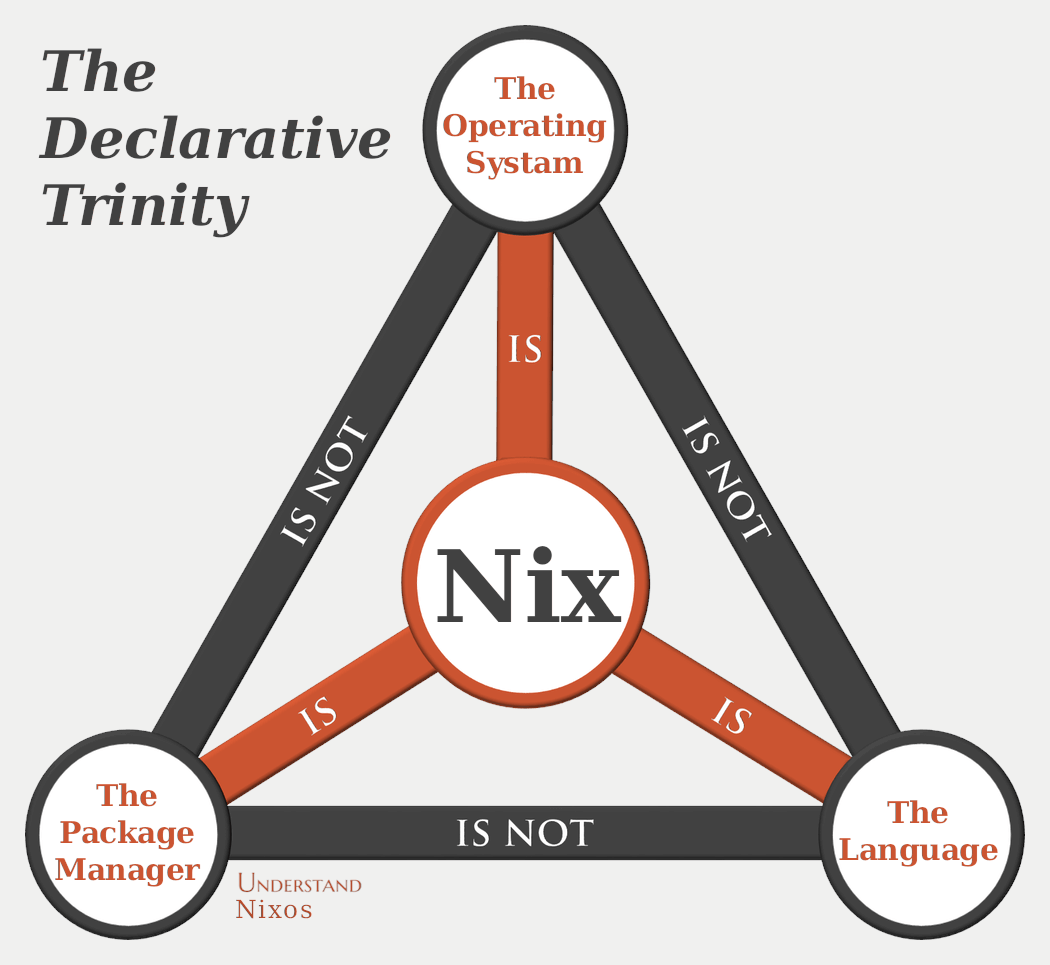
\includegraphics[width=0.6\textwidth]{nixgodhead.png}
\end{multicols}

\end{frame}

\begin{frame}[fragile]

\frametitle{What is Nix (the DSL)?}

Follow along: \href{https://glot.io/new/nix}{https://glot.io/new/nix} 

docker run -it ethancedwards8/nix

JSON like syntax :()
\begin{verbatim}
{
    string = "hello";
    integer = 1;
    float = 3.141;
    bool = true;
    nullval = null;
    list = [ 1 "two" false ];
    attribute-set = {
        a = { e = "hello"; };
        b = 2;
        c = 2.718;
        d = false;
    }; # comments are supported
}
\end{verbatim}

\end{frame}

\begin{frame}[fragile]

\frametitle{rec keyword/let blocks}

\begin{verbatim}
rec {
  one = 1;
  two = one + 1;
  three = two + 1;
}
# evals to:
{ one = 1; three = 3; two = 2; }


let
  b = a + 1;
  a = 1;
in
a + b
# evals to:
3
\end{verbatim}

\end{frame}


\begin{frame}[fragile]

\frametitle{with keyword}

\begin{verbatim}
let
  a = {
    x = 1;
    y = 2;
    z = 3;
  };
in
with a; [ x y z ]
# evals to
[ 1 2 3 ]
# with a; [ x y z ]
# is equivalent to
# [ a.x a.y a.z ]
\end{verbatim}

\end{frame}


\begin{frame}[fragile]

\frametitle{Functions!}

Nix has strong Functional Programming roots:
\begin{enumerate}
    \item Immutable variables
    \item Single argument functions (currying!)
    \item Lazy evaluation
    \item Anonymous, first-class functions
\end{enumerate}


\begin{verbatim}
# single argument functions
f = x: x + 1 # f 3 == 4

# single argument functions *with a set*
let
  f = {a, b}: a + b;
in
f { a = 1; b = 2; } # == 3
\end{verbatim}

Learn more at nix.dev

\end{frame}

\begin{frame}

\frametitle{Nix the package manager}

Now that you know the language, you can understand the package manager. The nix language is used to create "derivations," which are the basic building blocks of packages. A derivation essentially includes the instructions for building/compiling a program. (I'll show some code later)


Packages can depend on other packages (like libraries), creating dependency trees.

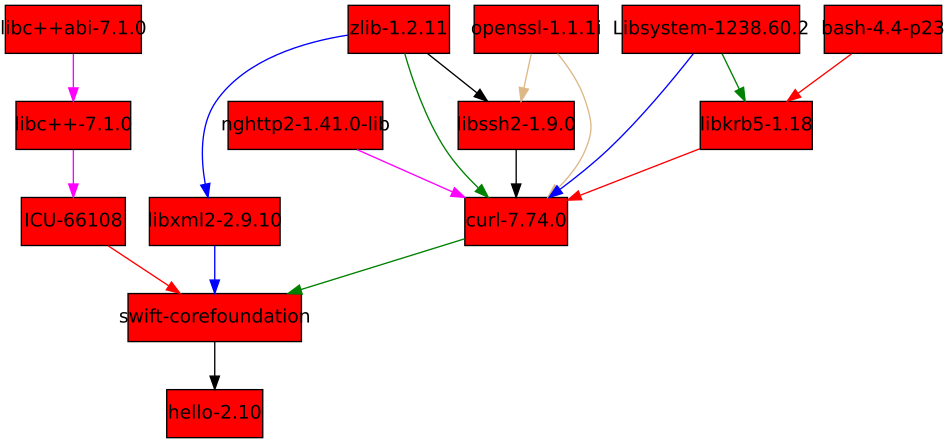
\includegraphics[width=0.6\textwidth]{depgraph.png}

\end{frame}

\begin{frame}

\frametitle{So, what's the point?}

Nix provides some guarantees that are pretty attractive to users: (buzzword warning)

\begin{enumerate}
    \item Determinism
    \item Reproducibility
    \item Build environments
    \item Rollbacks
    \item Declarative configurations!!!
\end{enumerate}

\end{frame}

\begin{frame}[fragile]

\frametitle{Nix managing packages}

Nix can be used to imperatively (bad) install packages or to declaratively (good) install them:

\begin{verbatim}
# flakes (new, more reproducible)
$ nix profile add nixpkgs#neovim
# channel (older)
$ nix-env -iA nixpkgs.hello

# declaratively in configuration.nix
environment.systemPackages = with pkgs; [
    neovim
];
\end{verbatim}

\end{frame}


\begin{frame}

\frametitle{Nixpkgs}

Nixpkgs is a collection of derivations that make up the Nixpkgs package set. We are the most up-to-date and largest package set in the world.

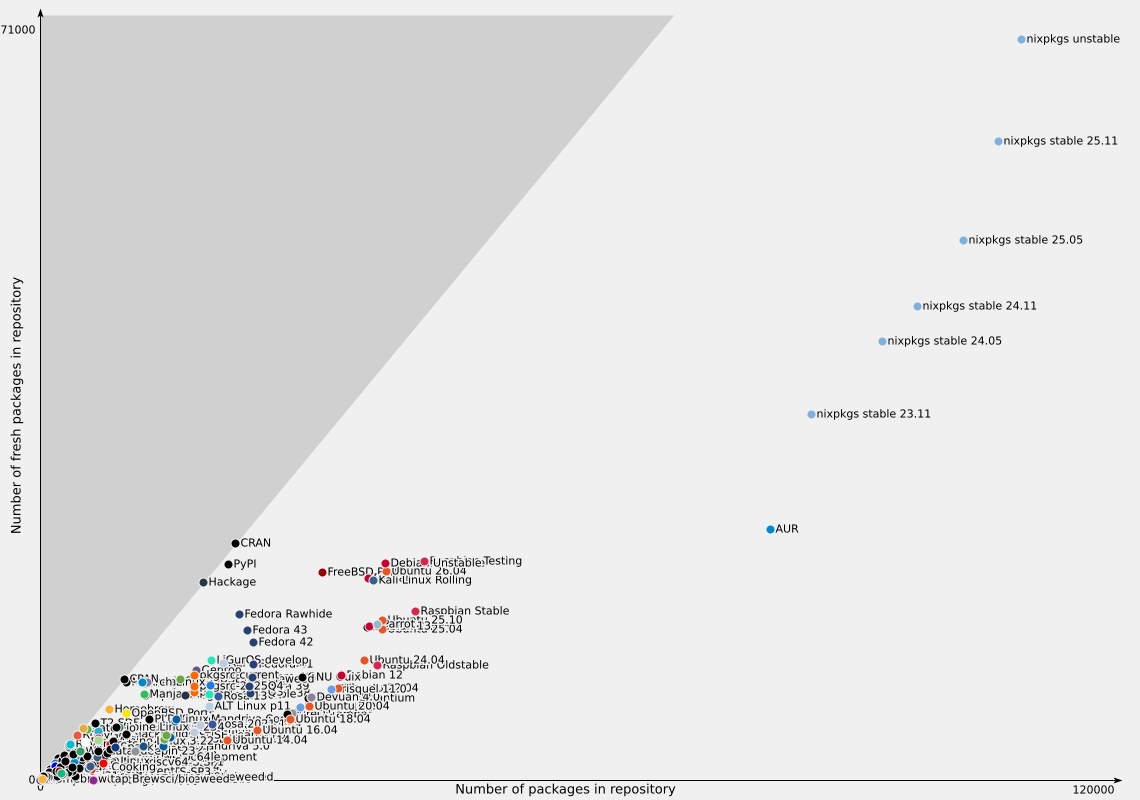
\includegraphics[width=0.6\textwidth]{repos.png}

This is achieved through insane levels of automation, testing, developer tooling, and more.

\end{frame}

\begin{frame}

\frametitle{Graphic}


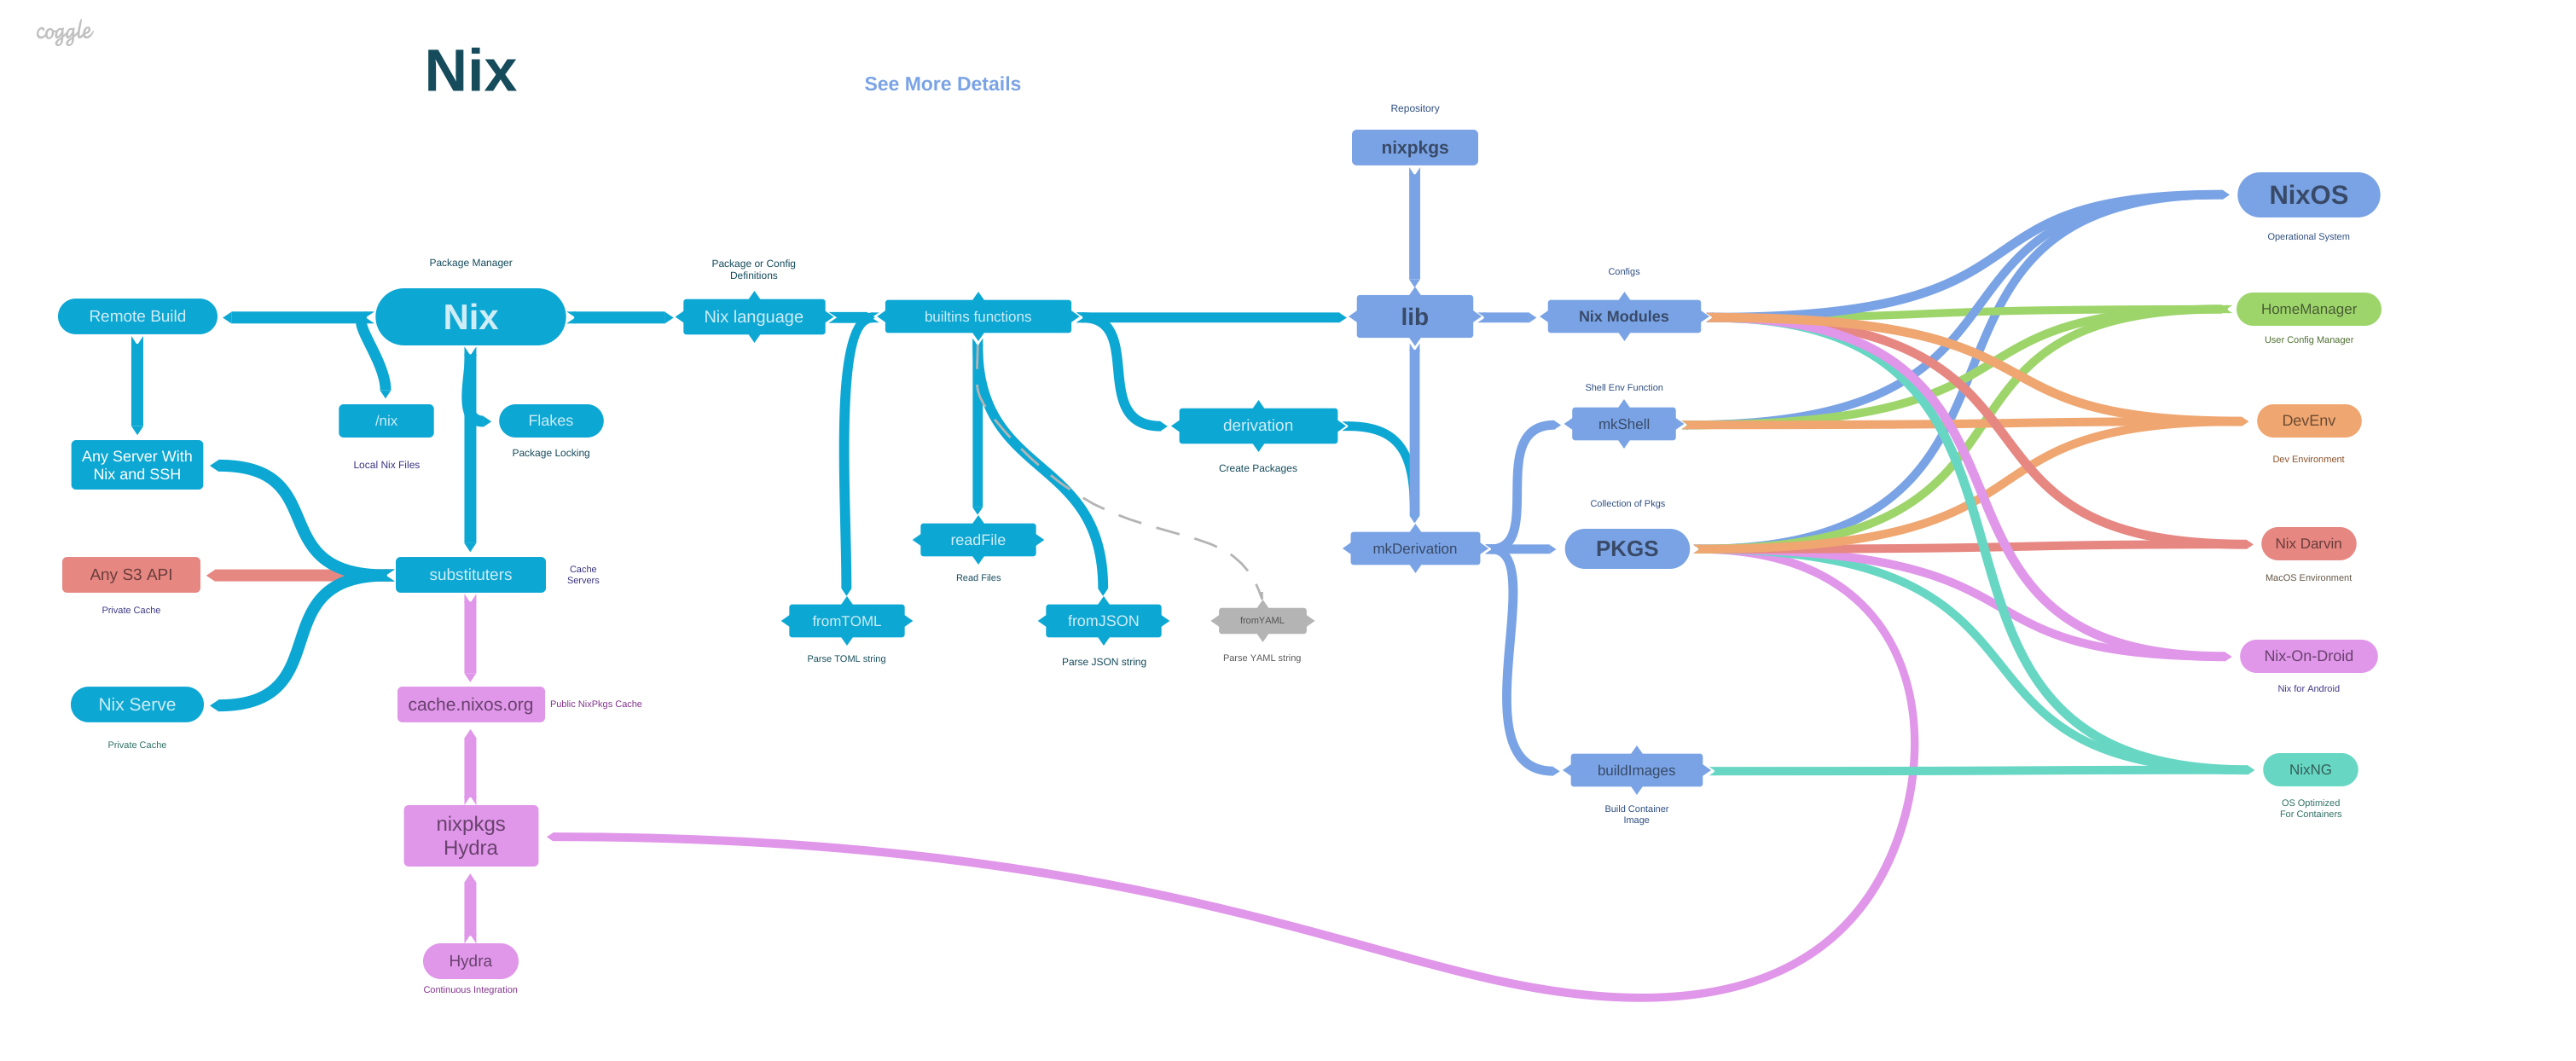
\includegraphics[width=1.1\textwidth]{nixgraph.png}


\end{frame}


\begin{frame}

\frametitle{NixOS}

NixOS is a Linux distribution built around Nix the package manager as well as Nixpkgs. It allows users to declaratively install packages like neovim, firefox, ghostty, etc. but also allows for users to install services like docker, nginx, nextcloud, and so much more. This is a bit hard to show in slides, let's do a demo!

\end{frame}

\begin{frame}

\frametitle{Flakes}

Flakes are the epitome of determinism!

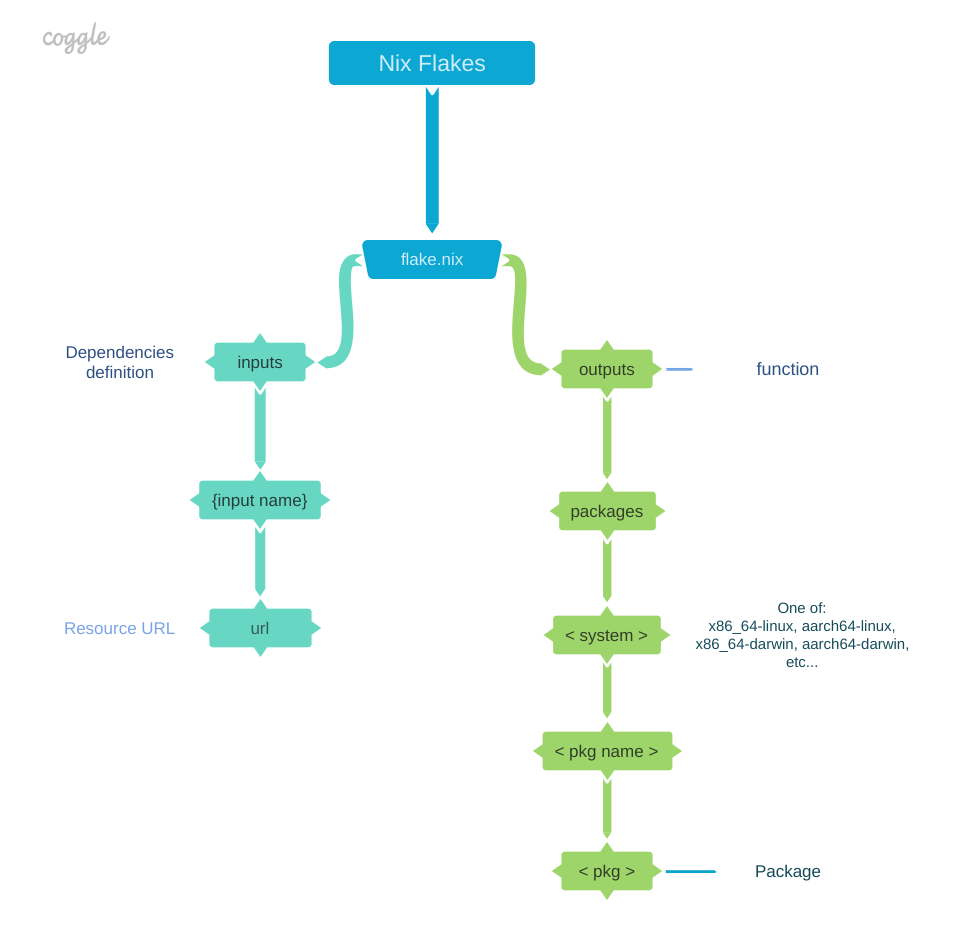
\includegraphics[width=.8\textwidth]{flakes.png}

\end{frame}

\begin{frame}[fragile]

\frametitle{Other builders: Docker}

Nix can even be used to build Docker images:

\begin{verbatim}
pkgs.dockerTools.buildImage {
  name = "nix-hello-image";
  tag = "latest";

  contents = pkgs.hello;

  config = {
    Cmd = [ "${pkgs.hello}/bin/hello" ];
    ExposedPorts = {};
  };
}
\end{verbatim}

\end{frame}

\begin{frame}[fragile]

\frametitle{Other builders: Cross Compilation}

Nix can also be used to cross compile packages to other platforms/architectures.

\begin{verbatim}
nix build nixpkgs#pkgsCross.aarch64-multiplatform.hello
\end{verbatim}

\end{frame}



\end{document}
